\begin{center}
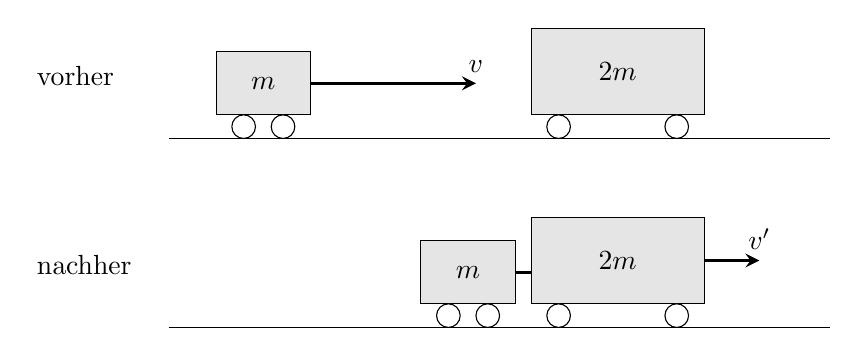
\begin{tikzpicture}[>=stealth]
 \node[anchor=west] at (0,0.8) {vorher};
 \draw (1.8,0) -- (10.2,0);
 \draw[fill=gray!20] (2.4,0.3) rectangle (3.6,1.1);
 \node at (3,0.7) {$m$};
 \draw[fill=white] (2.75,0.15) circle (0.15) (3.25,0.15) circle (0.15);
 \draw[->, very thick] (3.6,0.7) -- (5.7,0.7) node[above] {$v$};
 \draw[fill=gray!20] (6.4,0.3) rectangle (8.6,1.4);
 \node at (7.5,0.85) {$2m$};
 \draw[fill=white] (6.75,0.15) circle (0.15) (8.25,0.15) circle (0.15);
 \node[anchor=west] at (0,-1.6) {nachher};
 \draw (1.8,-2.4) -- (10.2,-2.4);
 \draw[fill=gray!20] (5,-2.1) rectangle (6.2,-1.3);
 \node at (5.6,-1.7) {$m$};
 \draw[fill=white] (5.35,-2.25) circle (0.15) (5.85,-2.25) circle (0.15);
 \draw[very thick] (6.2,-1.7) -- (6.4,-1.7);
 \draw[fill=gray!20] (6.4,-2.1) rectangle (8.6,-1);
 \node at (7.5,-1.55) {$2m$};
 \draw[fill=white] (6.75,-2.25) circle (0.15) (8.25,-2.25) circle (0.15);
 \draw[->, very thick] (8.6,-1.55) -- (9.3,-1.55) node[above] {$v'$};
\end{tikzpicture}
\end{center}

Impulserhaltung für die gemeinsame Geschwindigkeit $v'$:
\begin{align}
 m\,v &= \left(m+2m\right)v' \quad\Rightarrow\quad v' = \frac{v}{3}
\end{align}
Die kinetische Energie vor und nach dem Stoss ist
\begin{align}
 E &= \frac{1}{2}m\,v^2 \\
 E' &= \frac{1}{2}\cdot 3m\cdot\left(\frac{v}{3}\right)^2 = \frac{1}{6}m\,v^2
\end{align}
Erhalten bleibt also der Bruchteil
\begin{align}
 \frac{E'}{E} &= \frac{\frac{1}{6}m\,v^2}{\frac{1}{2}m\,v^2} = \result{\frac{1}{3}}
\end{align}
Zwei Drittel der mechanischen Energie werden in innere Energie umgewandelt.
